\documentclass{article}
\usepackage{graphicx} % Required for inserting images
\usepackage{amsmath}
\usepackage{amsfonts}
\usepackage{comment}
\usepackage{microtype}
\usepackage{bm}

\usepackage{mathtools}
\DeclarePairedDelimiter\bra{\langle}{\rvert}
\DeclarePairedDelimiter\ket{\lvert}{\rangle}
\DeclarePairedDelimiterX\braket[2]{\langle}{\rangle}{#1\,\delimsize\vert\,\mathopen{}#2}
\newcommand*\diff{\mathop{}\!\mathrm{d}}
\DeclarePairedDelimiterX\expval[3]{\langle}{\rangle}%
{#1\,\delimsize\vert\,\mathopen{}#2\,\delimsize\vert\,\mathopen{}#3}

\usepackage{hyperref}
\usepackage{xcolor}
\hypersetup{ % this is just my personal choice, feel free to change things
    colorlinks,
    linkcolor={red!50!black},
    citecolor={blue!50!black},
    urlcolor={blue!80!black},
}

\usepackage{simpler-wick}

\renewcommand\thesection{Part \alph{section})}  % chktex 9 % chktex 10 % tex-fmt: skip
\renewcommand\thesubsection{Solution} % tex-fmt: skip

\title{
    First midterm FYS4480\\
    Quantum mechanics for many-particle systems
}
\author{August Femtehjell}
\date{October 2024}

\begin{document}

\maketitle

\section*{Introduction}

In this midterm we will develop two simple models for studying the helium atom (with two electrons) and the beryllium atom with four electrons.

After having introduced the  Born-Oppenheimer approximation which effectively freezes out the nucleonic degrees of freedom, the Hamiltonian for \(N\) electrons takes the following form
\begin{equation*}
    \hat{H} = \sum_{i=1}^{N} t(x_i) - \sum_{i=1}^{N} k\frac{Ze^2}{r_i} + \sum_{i<j}^{N} \frac{ke^2}{r_{ij}},
\end{equation*}
with \(k=1.44\) eVnm.
Throughout this work we will use atomic units, this means that \(\hbar = c = e = m_e = 1\).
The constant \(k\) becomes also equal 1.
The resulting energies have to be multiplied by \(2 \times 13.6\) eV in order to obtain energies in eletronvolts.

We can rewrite our Hamiltonians as
\begin{equation}
    \hat{H} = \hat{H_0} + \hat{H_I}
    = \sum_{i=1}^{N}\hat{h}_0(x_i) + \sum_{i<j}^{N}\frac{1}{r_{ij}},
    \label{eq:H1H2}
\end{equation}
where  we have defined \(r_{ij} = |\bm{r}_i - \bm{r}_j|\) and \(\hat{h}_0(x_i) =  \hat{t}(x_i) - \frac{Z}{r_i}\).

The variable \(x\) contains both the spatial coordinates and the spin values.
The first term of Eq.~\eqref{eq:H1H2}, \(H_0\), is the sum of the \(N\) \emph{one-body} Hamiltonians \(\hat{h}_0\).
Each individual Hamiltonian \(\hat{h}_0\) contains the kinetic energy operator of an electron and its potential energy due to the attraction of the nucleus.
The second term, \(H_I\), is the sum of the \(N(N-1)/2\) two-body interactions between each pair of electrons.
Note that the double sum carries a restriction \(i<j\).

As basis functions for our calculations we will use hydrogen-like single-particle functions.
This means the onebody operator is diagonal in this basis for states \(i,j\) with quantum numbers
\(n,l,m_l,s,m_s\) with energies
\begin{equation}
    \expval{i}{\hat{h}_0}{j} = -\frac{Z^2}{2n^2}\delta_{ij}.
    \label{eq:onebody}
\end{equation}
The quantum number \(n\) refers to the number of nodes of the wave function.
Observe that this expectation value is independent of spin.

We will in all calculations here restrict ourselves to only so-called \(s\)-waves, that is the orbital momentum \(l\) is zero.
We will also limit the quantum number \(n\) to \(n \le 3\).
It means that every \(ns\) state can accommodate two electrons due to the spin degeneracy.

In the calculations you will need the Coulomb interaction with matrix elements involving single-particle wave functions with \(l = 0\) only, the
so-called \(s\)-waves.
We need only the radial part since the spherical harmonics for the \(s\)-waves are rather simple.
We omit single-particle states with \(l > 0\).
The actual integrals we need, are tabulated at the end.
Our radial wave functions are
\begin{equation*}
    R_{n0}(r) = \left( \frac{2Z}{n} \right)^{3/2} \sqrt{\frac{(n-1)!}{2n\times n!}} L_{n-1}^1 \left( \frac{2Zr}{n} \right) \exp{\left( -\frac{Zr}{n} \right)},
\end{equation*}
where \(L_{n-1}^1(r)\) are the so-called Laguerre polynomials.
These wave functions can then be used to compute the direct part of the Coulomb interaction
\begin{equation*}
    \expval*{\alpha\beta}{V}{\gamma\delta} = \int r_1^2 dr_1 \int r_2^2 dr_2 R_{n_{\alpha} 0}^*(r_1) R_{n_{\beta} 0}^*(r_2) \frac{1}{r_{12}}R_{n_{\gamma} 0}(r_1) R_{n_{\delta} 0}(r_2).
\end{equation*}

Observe that this is only the radial integral and that the labels \( \alpha,\beta,\gamma,\delta \) refer only to the quantum numbers \(n,l,m_l\), with \(m_l\) the projection of the orbital momentum \(l\).
A similar expression can be found for the exchange part.
Since we have restricted ourselves to only \(s\)-waves, these integrals are straightforward but tedious to calculate.
As an addendum to this midterm we list all closed-form expressions for the relevant matrix elements.
Note well that these matrix elements do not include spin.
When setting up the final antisymmetrized matrix elements you need to consider the spin degrees of freedom as well.
Please pay in particular attention to the exchange part and the pertinent spin values of the single-particle states.

We will also, for both helium and beryllium assume that the many-particle states we construct have always the same total spin projection \(M_S = 0\).
This means that if we excite one or two particles from the ground state, the spins of the various single-particle states should always sum up to zero.

\section{Setting up the basis}
We start with the helium atom and define our single-particle Hilbert
space to consist of the single-particle orbits \(1s\), \(2s\) and \(3s\),
with their corresponding spin degeneracies.

Set up the ansatz for the ground state \(\ket*{c} = \ket*{\Phi_0}\) in second quantization.
Define the second quantization and define a table of single-particle states.
Construct thereafter all possible one-particle-one-hole
excitations \(\ket*{\Phi_i^a}\) where \(i\) refer to levels below the Fermi level (define this level) and \(a\) refers to particle states.
Define particles and holes.
The Slater determinants have to be written in terms of the respective creation and annihilation operators.
The states you construct should all have total spin projection \(M_S=0\).
Construct also all possible two-particle-two-hole states \(\ket*{\Phi_{ij}^{ab}}\) in a second quantization
representation.

\subsection{}
We define the Fermi level as \(1s\), such that the ground state is given by
\begin{equation}
    \ket*{\Phi_0} = \ket*{c} = a_{1\sigma_1}^\dagger a_{1\sigma_2}^\dagger \ket*{0},
\end{equation}
where we define $\sigma_1 = \ \uparrow \ = +1/2$ and $\sigma_2 = \ \downarrow \ = -1/2$.
Here, we define particles as electrons (?) above the Fermi level, and holes as the lack of electrons in slots below the Fermi level.

In order to have a one-particle-one-hole excitation, the spin in the hole and particle states must match.
All possible one-particle-one-hole (1p1h) excitations are then
\begin{align*}
    \ket*{\Phi_{1\sigma_1}^{2\sigma_1}} &= a_{2\sigma_1}^\dagger a_{1\sigma_1} \ket*{\Phi_0}, &
    \ket*{\Phi_{1\sigma_1}^{3\sigma_1}} &= a_{3\sigma_1}^\dagger a_{1\sigma_1} \ket*{\Phi_0}, \\
    \ket*{\Phi_{1\sigma_2}^{2\sigma_2}} &= a_{2\sigma_2}^\dagger a_{1\sigma_2} \ket*{\Phi_0}, &
    \ket*{\Phi_{1\sigma_2}^{3\sigma_2}} &= a_{3\sigma_2}^\dagger a_{1\sigma_2} \ket*{\Phi_0},
\end{align*}
where we always excite a particle from the $1s$ state, to the higher states, with the same spin such that $M_S = 0$.

For the possible two-particle-two-hole (2p2h) excitations $\ket*{\Phi_{ij}^{ab}}$, we have that both electrons below the Fermi level excite, and that the particles above the Fermi level have opposite spins.
We then have that the possible configurations are
\begin{align*}
    \ket*{\Phi_{1\sigma_1, 1\sigma_2}^{2\sigma_1, 2\sigma_2}} &= a_{2\sigma_1}^\dagger a_{2\sigma_2}^\dagger a_{1\sigma_2} a_{1\sigma_1} \ket*{\Phi_0}, &
    \ket*{\Phi_{1\sigma_1, 1\sigma_2}^{2\sigma_1, 3\sigma_2}} &= a_{2\sigma_1}^\dagger a_{3\sigma_2}^\dagger a_{1\sigma_2} a_{1\sigma_1} \ket*{\Phi_0}, \\
    \ket*{\Phi_{1\sigma_1, 1\sigma_2}^{3\sigma_1, 2\sigma_2}} &= a_{3\sigma_1}^\dagger a_{2\sigma_2}^\dagger a_{1\sigma_2} a_{1\sigma_1} \ket*{\Phi_0}, &
    \ket*{\Phi_{1\sigma_1, 1\sigma_2}^{3\sigma_1, 3\sigma_2}} &= a_{3\sigma_1}^\dagger a_{3\sigma_2}^\dagger a_{1\sigma_2} a_{1\sigma_1} \ket*{\Phi_0}.
\end{align*}



\section{Second quantized Hamiltonian}
Define the Hamiltonian in a second-quantized form and use this to compute the expectation value of the ground state (defining the so-called reference energy and later our Hartree-Fock functional) of
the helium atom.
Show that it is given by
\begin{equation}
    E[\Phi_0] = \expval{c}{\hat{H}}{c} = \sum_{i} \expval{i}{\hat{h}_0}{i} + \frac{1}{2} \sum_{ij} \left[\expval*{ij}{\frac{1}{r_{ij}}}{ij} - \expval*{ij}{\frac{1}{r_{ij}}}{ji}\right].
\end{equation}
Define properly the sums keeping in mind that the states $ij$ refer to all quantum numbers $n, l, m_l, s, m_s$.
Use the values for the various matrix elements listed at the end of the midterm to find the value of $E$ as function of $Z$ and compute $E$ as function of $Z$.

\subsection{}
We consider the Hamiltonian $\hat{H} = \hat{H}_0 + \hat{H}_I$, where $\hat{H}_0$ is the one-body part and $\hat{H}_I$ is the two-body part, given by
\begin{align*}
    \hat{H}_0 &= \sum_{i=1}^{N}\hat{h}_0(x_i), &
    \hat{H}_I &= \sum_{i<j}^{N}\frac{1}{r_{ij}}.
\end{align*}
In second quantization, we rewrite the one-body part as
\begin{equation}
    \hat{H}_0 = \sum_{\alpha\beta} \expval{\alpha}{\hat{h}_0}{\beta} a_\alpha^\dagger a_\beta.
\end{equation}
With the new annihilation and creation operators $b_\alpha$ and $b_\alpha^\dagger$ with respect to the new vacuum state $\ket*{\Phi_0}$, we can rewrite this as
\begin{equation}\label{eq:H0_second_quant}
    \begin{split}
        \hat{H}_0 =& \sum_{ab} \expval{a}{\hat{h}_0}{b} b_a^\dagger b_b + \sum_{ai} \left[ \expval{a}{\hat{h}_0}{i} b_a^\dagger b_i^\dagger + \expval{i}{\hat{h}_0}{a} b_i b_a \right] \\
        &+ \sum_{i} \expval{i}{\hat{h}_0}{i} - \sum_{ij} \expval{j}{\hat{h}_0}{i} b_i^\dagger b_j.
    \end{split}
\end{equation}

Recalling that
\begin{equation*}
    \expval{\alpha}{\hat{h}_0}{\beta} = -\frac{Z^2}{2n^2}\delta_{\alpha \beta},
\end{equation*}
we can simplify the expression to
\begin{equation}\label{eq:H0_second_quant_simple}
    \hat{H}_0 = \sum_{a} \expval{a}{\hat{h}_0}{a} b_a^\dagger b_a + \sum_{i} \expval{i}{\hat{h}_0}{i} - \sum_{i} \expval{i}{\hat{h}_0}{i} b_i^\dagger b_i.
\end{equation}
The first and last terms vanish, as both $b_\alpha \ket*{\Phi_0} = 0$, leaving us with
\begin{equation}
    \expval{c}{\hat{H}_0}{c} = \sum_{i} \expval{i}{\hat{h}_0}{i} \braket{c}{c} =: \mathcal{E}_0^{\text{Ref}}.
\end{equation}

The two-body part is rewritten in second quantization as
\begin{equation}
    \hat{H}_I = \frac{1}{2} \sum_{\alpha \beta \gamma \delta} \expval{\alpha \beta}{V}{\gamma \delta} a_\alpha^\dagger a_\beta^\dagger a_\delta a_\gamma.
\end{equation}
With the new annihilation and creation operators, we can rewrite this as
\begin{equation*}
    \hat{H}_I = \hat{H}_I^{(1)} + \hat{H}_I^{(2)} + \hat{H}_I^{(3)} + \hat{H}_I^{(4)} + \hat{H}_I^{(5)},
\end{equation*}
where utilizing antisymmetrized matrix elements for the sake of brevity, we have
\begin{align*}
    \hat{H}_I^{(1)} &= \frac{1}{4} \sum_{abcd} \expval{ab}{V}{cd} b_a^\dagger b_b^\dagger b_d b_c, \\
    \hat{H}_I^{(2)} &= \frac{1}{4} \sum_{abci} \expval{ab}{V}{ci} b_a^\dagger b_b^\dagger b_i^\dagger b_c + \expval{ai}{V}{cb} b_a^\dagger b_i b_b b_c \\
    \hat{H}_I^{(3)} &= \frac{1}{4} \sum_{abij} \left[\expval{ab}{V}{ij} b_a^\dagger b_b^\dagger b_j^\dagger b_i^\dagger + \expval{ij}{V}{ab} b_a b_b b_j b_i \right] \\
    &\qquad + \frac{1}{2} \sum_{abij} \expval{ai}{V}{bj} b_a^\dagger b_j^\dagger b_b b_i + \frac{1}{2} \sum_{abi} \expval{ai}{V}{bi} b_a^\dagger b_b \\
    \hat{H}_I^{(4)} &= \frac{1}{4} \sum_{aijk} \left[ \expval{ai}{V}{jk} b_a^\dagger b_k^\dagger b_j^\dagger b_i + \expval{ji}{V}{ak} b_k^\dagger b_j b_i b_a \right] \\
    &\qquad + \frac{1}{2} \sum_{aij} \left[ \expval{ai}{V}{ji} b_a^\dagger b_j^\dagger + \expval{ji}{V}{ai} b_j b_a \right] \\
    \hat{H}_I^{(5)} &= \frac{1}{4} \sum_{ijkl} \expval{kl}{V}{ij} b_i^\dagger b_j^\dagger b_l b_k + \frac{1}{2} \sum_{ijk} \expval{ij}{V}{kj} b_k^\dagger b_i + \frac{1}{2} \sum_{ij} \expval{ij}{V}{ij}.
\end{align*}

In order to simplify the computations later, we briefly summarize the qualitative properties of each of the terms above.
\begin{enumerate}[(1).]
    \item Contributes for $\geq$two-particle states
    \item Creates or removes a three-particle-one-hole state, while conserving the number of particles
    \item Term by term,
        \begin{enumerate}
            \item Creates a two-particle-two-hole state by either removing two particles and creating two holes, or by removing two holes and creating two particles.
            \item Creates two one-particle-one-hole pairs.
            \item Contributions between particle pairs, and the hole states.
        \end{enumerate}
    \item Term by term,
        \begin{enumerate}
            \item Creation of a one-particle-one-hole pair, interacting with a hole.
            \item One-particle-one-hole pair interacting with a hole.
        \end{enumerate}
    \item Term by term,
        \begin{enumerate}
            \item Interactions between pairs of two hole states.
            \item Interactions between a hole and the other holes.
            \item Energy from the ground state.
        \end{enumerate}
\end{enumerate}

\begin{comment}
    In terms of the ground state, we only have contributions from the terms involving $b_{\alpha}^\dagger$.
    Everything else vanishes.
    \begin{enumerate}[(1.)]
        \item No contribution $b_c \ket*{\Phi_0} = 0$
        \item No contribution $b_c \ket*{\Phi_0} = 0$
        \item
            \begin{enumerate}[(a)]
                \item No contribution by orthogonality
                \item No contribution $b_i \ket*{\Phi_0} = 0$
                \item No contribution $b_b \ket*{\Phi_0} = 0$
            \end{enumerate}
        \item
            \begin{enumerate}[(a)]
                \item No contribution $b_i \ket*{\Phi_0} = 0$ and $b_a \ket*{\Phi_0} = 0$
                \item No contribution orthogonality, and lack of one-particle-one-hole states
            \end{enumerate}
        \item
            \begin{enumerate}
                \item
            \end{enumerate}
    \end{enumerate}
\end{comment}

We can now quickly see that $\expval{c}{\hat{H}_I}{c}$ only gets a contribution from the last $H_I^{(5)}$ term, as the other terms vanish due to either an annihilation operator acting on the vacuum state, or orthogonality of the states created.
We are then just left with
\begin{equation}
    \expval{\Phi_0}{\hat{H}_I}{\Phi_0} = \frac{1}{2} \sum_{ij} \expval{ij}{V}{ij}_{AS} = \frac{1}{2} \sum_{ij} \expval{ij}{V}{ij} - \expval{ij}{V}{ji} = \mathcal{E}_I^{\text{Ref}}.
\end{equation}

Finally, combining this with the expectation value of the one-body part, we get that the complete expectation value of the ground state is
\begin{equation}
    E[\Phi_0]
    = \expval{c}{\hat{H}}{c}
    = \sum_{i} \expval{i}{\hat{h}_0}{i} + \frac{1}{2} \sum_{\substack{ij \\ i \neq j}} \left[\expval*{ij}{\frac{1}{r_{ij}}}{ij} - \expval*{ij}{\frac{1}{r_{ij}}}{ji}\right],
\end{equation}
as we wanted to show.

\begin{comment}
    Computing the results of $\expval{\Phi_0}{\hat{H}_I^{(5)}}{\Phi_0}$ term by term, we get the possible contractions
    \begin{equation*}
        \arraycolsep=1.4pt
        \begin{array}{ccrcccr}
            \langle \Phi_0 \vert
            \wick
            {
                \c2 b_i^\dagger
                \c1 b_j^\dagger
                \c1 b_l
                \c2 b_k
            }
            \vert \Phi_0 \rangle
            &=& \delta_{i k} \delta_{j l} &\implies& &&  \expval{i j}{V}{i j},  \\
            \langle \Phi_0 \vert
            \wick
            {
                \c1 b_i^\dagger
                \c2 b_j^\dagger
                \c1 b_l
                \c2 b_k
            }
            \vert \Phi_0 \rangle
            &=& -\delta_{i l} \delta_{j k} &\implies& -\expval{j i}{V}{i j} &= &-\expval{i j}{V}{j i}, \\
        \end{array}
    \end{equation*}
    from the first term.
    For the second we just get $\delta_{ik}$, giving us a term $\frac{1}{2} \sum_{ij} \expval{ij}{V}{ij}$.
    This leaves us with the expectation value of the two-body part as
    \begin{align*}
        \expval{\Phi_0}{\hat{H}_I}{\Phi_0} &= \expval{\Phi_0}{\hat{H}_I^{(5)}}{\Phi_0} \\
        &= \sum_{ij} \frac{1}{4} \left[ \expval{i j}{V}{i j} - \expval{i j}{V}{j i} \right] + \frac{1}{2} \sum_{ij} \expval{ij}{V}{ij} + \frac{1}{2} \sum_{ij} \expval{ij}{V}{ij} \\
    \end{align*}
\end{comment}
\begin{comment}
    \newpage

    Then, the expectation value of the ground state with the one-body part is given by
    \begin{equation*}
        \expval{\Phi_0}{\hat{H}_0}{\Phi_0} = \sum_{\alpha\beta} \expval{\alpha}{\hat{h}_0}{\beta} \expval{\Phi_0}{a_\alpha^\dagger a_\beta}{\Phi_0}.
    \end{equation*}
    For all states where either $\alpha > F, \beta > F$, we have that $\expval{\Phi_0}{a_\alpha^\dagger a_\beta}{\Phi_0} = 0$.
    Thus, the sum is restricted to $i,j \le F$,
    \begin{align*}
        \expval{\Phi_0}{\hat{H}_0}{\Phi_0} &= \sum_{ij} \expval{i}{\hat{h}_0}{j} \expval{\Phi_0}{a_i^\dagger a_j}{\Phi_0} \\
        &= \sum_{ij} \expval{i}{\hat{h}_0}{j} \delta_{ij} \\
        &= \sum_{i} \expval{i}{\hat{h}_0}{i},
    \end{align*}
    where we utilized the orthonormality of the single-particle states.

    The two-body part is rewritten in second quantization as
    \begin{equation*}
        \hat{H}_I = \frac{1}{2} \sum_{\alpha \beta \gamma \delta} \expval{\alpha \beta}{V}{\gamma \delta} a_\alpha^\dagger a_\beta^\dagger a_\delta a_\gamma.
    \end{equation*}
    The expectation value of the ground state with the two-body part is then
    \begin{equation*}
        \expval{\Phi_0}{\hat{H}_I}{\Phi_0} = \frac{1}{2} \sum_{\alpha\beta\gamma\delta} \expval{\alpha\beta}{V}{\gamma\delta} \expval{\Phi_0}{a_\alpha^\dagger a_\beta^\dagger a_\delta a_\gamma}{\Phi_0}.
    \end{equation*}
    The possible contributing contractions are
    \begin{align*}
        \wick{\c2 a_\alpha^\dagger \c1 a_\beta^\dagger \c1 a_\delta \c2 a_\gamma} &= \delta_{\alpha\gamma} \delta_{\beta\delta}, &
        \wick{\c1 a_\alpha^\dagger \c2 a_\beta^\dagger \c1 a_\delta \c2 a_\gamma} &= -\delta_{\alpha\delta} \delta_{\beta\gamma}. \\
    \end{align*}
    Whenever $\alpha > F$ or $\beta > F$, the expectation value vanishes, so we relabel the summation to $i, j$. The terms also vanish if $i = j$. % TODO: Reword maybe
    We are then left with
    \begin{equation*}
        \expval{\Phi_0}{\hat{H}_0}{\Phi_0} = \frac{1}{2} \sum_{\substack{ij \\ i \neq j}} \expval*{ij}{V}{ij} - \expval*{ij}{V}{ji}.
    \end{equation*}

    Gathering this, we get that the complete expectation value of the ground state is
    \begin{equation}
        E[\Phi_0]
        = \expval{c}{\hat{H}}{c}
        = \sum_{i} \expval{i}{\hat{h}_0}{i} + \frac{1}{2} \sum_{\substack{ij \\ i \neq j}} \expval*{ij}{\frac{1}{r_{ij}}}{ij} - \expval*{ij}{\frac{1}{r_{ij}}}{ji},
    \end{equation}
    as we wanted to show.
\end{comment}

In the case of the electrons in the helium atom, we only have $n = 1$, $l = 0$, differing only in the spin quantum number $m_s = \pm 1/2$.
The expectation value of the one-body part is then
\begin{equation*}
    \expval{\Phi_0}{\hat{H}_0}{\Phi_0} = \sum_{\sigma \in \{\pm 1/2\}} \expval{1\sigma}{\hat{h}_0}{1\sigma} = -Z^2,
\end{equation*}
and the expectation value of the two-body part is, writing just $\sigma_{+}$ and $\sigma_{-}$ for the spins with $n = 1$,
\begin{equation*}
    \expval{\Phi_0}{\hat{H}_I}{\Phi_0}
    = \frac{1}{2} \sum_{\substack{\sigma_{+}\sigma_{-}\\ \sigma_{+} \neq \sigma_{-}}}
    \underbrace{\expval*{\sigma_{+} \sigma_{-}}{\frac{1}{r_{\sigma_{+}\sigma_{-}}}}{\sigma_{+} \sigma_{-}}}_{\textnormal{Direct term}}
    - \underbrace{\expval*{\sigma_{+} \sigma_{-}}{\frac{1}{r_{\sigma_{+}\sigma_{-}}}}{\sigma_{-}\sigma_{+}}}_{\textnormal{Exchange term}}.
\end{equation*}
The exchange term vanishes since the states are orthogonal, and we are left with the direct term.
We are then just left with
\begin{equation*}
    \expval{\Phi_0}{\hat{H}_I}{\Phi_0} = \frac{1}{2}\left[ \expval*{\sigma_{+} \sigma_{-}}{\frac{1}{r_{\sigma_{+} \sigma_{-}}}}{\sigma_{+} \sigma_{-}} + \expval*{\sigma_{-} \sigma_{+}}{\frac{1}{r_{\sigma_{+} \sigma_{-}}}}{\sigma_{-} \sigma_{+}}\right].
\end{equation*}
As $\hat{H}_I$ is invariant under the change of label $\sigma$, we can simplify this to
\begin{equation*}
    \expval{\Phi_0}{\hat{H}_I}{\Phi_0} = \expval*{\sigma_{+} \sigma_{-}}{\frac{1}{r_{\sigma_{+} \sigma_{-}}}}{\sigma_{+} \sigma_{-}} = \frac{5}{8} Z.
\end{equation*}

Combining this, we find that the expectation value of the ground state is
\begin{equation}
    E[\Phi_0] = -Z^2 + \tfrac{5}{8}Z,
\end{equation}
which as a function of $Z$ is shown in \autoref{fig:energy}.

\begin{figure}[ht]
    \centering
    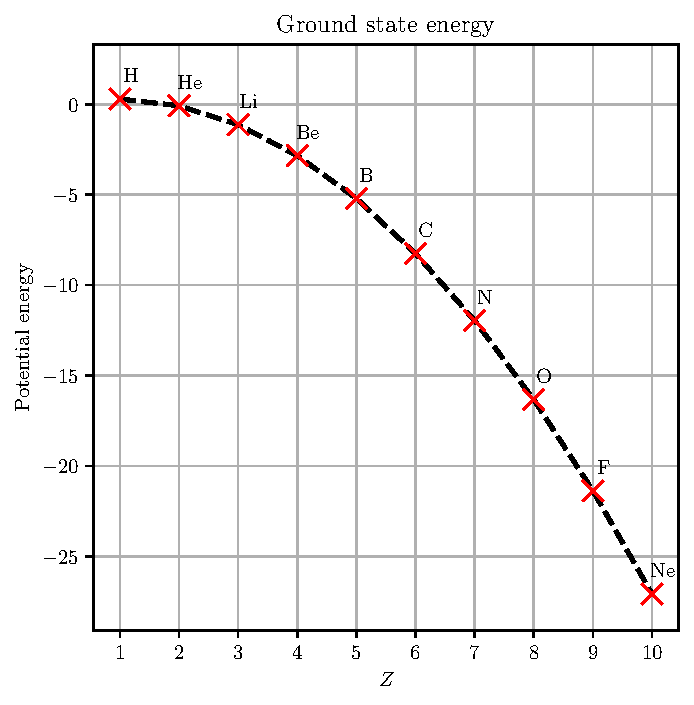
\includegraphics{figs/energy_plot.pdf}
    \caption{The expectation value of the ground states of an atom with two electrons as a function of the nuclear charge $Z$.\label{fig:energy}}
\end{figure}


\section{Limiting ourselves to one-particle-one excitations}
Hereafter we will limit ourselves to a system which now contains only one-particle-one-hole excitations beyond the chosen state $\ket{c}$.
Using the possible Slater determinants from exercise a) for the helium atom, find the expressions (without inserting the explicit values for the matrix elements first) for % chktex 10 % tex-fmt: skip
\begin{equation*}
    \expval{c}{\hat{H}}{\Phi_i^a},
\end{equation*}
and
\begin{equation*}
    \expval{\Phi_i^a}{\hat{H}}{\Phi_j^b}.
\end{equation*}
Represent these expressions in a diagrammatic form, both for the onebody part and the two-body part of the Hamiltonian.

Insert then the explicit values for the various matrix elements and set up the final Hamiltonian matrix and diagonalize it using for example Python as programming language.
Compare your results from those of exercise b) and comment your results. % chktex 10 % tex-fmt: skip

The exact energy with our Hamiltonian is $-2.9037$ atomic units for helium.
This value is also close to the experimental energy.

\subsection{}
We start by finding the value of the expression $\expval{c}{\hat{H}}{\Phi_i^a}$.
Writing out the terms, we have
\begin{align*}
    \expval{c}{\hat{H}}{\Phi_i^a} &= \expval{c}{\hat{H}_0 + \hat{H}_I}{\Phi_i^a} \\
    &= \expval{c}{\hat{H}_0}{\Phi_i^a} + \expval{c}{\hat{H}_I}{\Phi_i^a}.
\end{align*}
We can now read from Eq.~\eqref{eq:H0_second_quant} that the one-body part of the expression vanishes, either through an unmatched $b_\alpha^\dagger$ or simply $\braket{c}{\Phi_i^a} = 0$.
This gives us
\begin{equation}\label{eq:1p1h-ground-onebody}
    \expval{c}{\hat{H}_0}{\Phi_i^a} = 0.
\end{equation}

In order to make sure the number of annihilation and creation terms are correct, the contributing terms from $H_I$ are those with two more annihilation operators than creation operators, while also matching the number of holes and particles created.
We can then quickly reduce the possible contributing candidates to
\begin{equation*}
    \frac{1}{4} \sum_{aijk} \expval{ji}{V}{ak} b_k^\dagger b_j b_i b_a, \qquad
    \frac{1}{2} \sum_{aij} \expval{ji}{V}{ai} b_j b_a, \qquad
    \text{and} \qquad \mathcal{E}_I^\text{Ref}.
\end{equation*}
On closer inspection, we see that the first term vanishes, as $b_k^\dagger$ is unmatched, while the last term vanished due to $\braket{c}{\Phi_i^a} = 0$.

We then just need to evaluate the contractions of the second term, changing the labels of the sum $(a, i, j) \mapsto (b, j, k)$ to avoid confusion with $\ket{\Phi_i^a}$, which simply is
\begin{equation*}
    \langle c \vert
    \wick{
        \c2 b_k \c1 b_b \c1 b_a^\dagger \c2 b_i^\dagger
    }
    \vert c \rangle
    = \delta_{ik} \delta_{ab}.
\end{equation*}
We then get
\begin{equation}\label{eq:1p1h-ground-twobody}
    \expval*{c}{\hat{H}_I}{\Phi_i^a} = \frac{1}{2} \sum_{j} \expval{i j}{V}{a j}_{AS},
\end{equation}
taking into account that the matrix element in the sum is antisymmetrized.
Now, considering spin, the exchange term vanishes, leaving us with two times the direct term.
This gives us the final expression
\begin{equation}\label{eq:1p1h-ground}
    \expval{c}{\hat{H}}{\Phi_i^a} = \sum_{ij} \expval{ij}{V}{aj}.
\end{equation}

In the case of the helium atom, the only possible value for $j$ when $i = 1_{\sigma_1}$ is $j = 1_{\sigma_2}$.
Inserting for the explicit excitations, we get
\begin{equation}\label{eq:1p1h-ground-list}
    \arraycolsep=1.4pt
    \begin{array}{crcl}
        j = 1_{-}: \quad
        & \expval*{c}{\hat{H}}{\Phi_{1_{+}}^{2_{+}}}\hspace{0.27pt}
        & = &
        \expval{1_{-} 1_{+}}{V}{1_{-} 2_{+}} \\

        j = 1_{-}: \quad
        & \expval*{c}{\hat{H}}{\Phi_{1_{+}}^{3_{+}}}\hspace{0.27pt}
        & = &
        \expval{1_{-} 1_{+}}{V}{1_{-} 3_{+}} \\

        j = 1_{+}: \quad
        & \expval*{c}{\hat{H}}{\Phi_{1_{-}}^{2_{-}}}
        & = &
        \expval{1_{+} 1_{-}}{V}{1_{+} 2_{-}} \\

        j = 1_{+}: \quad
        & \expval*{c}{\hat{H}}{\Phi_{1_{-}}^{3_{-}}}
        & = &
        \expval{1_{+} 1_{-}}{V}{1_{+} 3_{-}}
    \end{array}
\end{equation}

Next, we find a simplified expression for $\expval{\Phi_i^a}{\hat{H}}{\Phi_j^b}$,
noting that
\begin{equation*}
    \expval{\Phi_i^a}{\hat{H}}{\Phi_j^b} = \expval{c}{b_i b_a \hat{H} b_b^\dagger b_j^\dagger}{c}.
\end{equation*}
Beginning again with the one-body part of the Hamiltonian, we have can read from Eq.~\eqref{eq:H0_second_quant_simple} that if $(i, a) \neq (j, b)$, the expression vanishes.
If however the pair is equal, we get a contribution, giving us
\begin{equation*}
    \expval{\Phi_i^a}{\hat{H}_0}{\Phi_j^b} = \delta_{ij} \delta_{ab} \left[ \expval{a}{\hat{h}_0}{a} - \expval{i}{\hat{h}_0}{i} + \mathcal{E}_0^{\text{Ref}} \right]
\end{equation*}

For the two-body part, we have that the possible contributing terms must then have an equal number of annihilation and creation operators in order to not vanish, reducing the candidates to
\begin{multicols}{2}{}
    \begin{enumerate}
        \item  $\displaystyle\frac{1}{4} \sum_{abcd} \expval{ab}{V}{cd} b_a^\dagger b_b^\dagger b_d b_c$
        \item  $\displaystyle\frac{1}{2} \sum_{abij} \expval{ai}{V}{bj} b_a^\dagger b_j^\dagger b_b b_i$
        \item  $\displaystyle\frac{1}{2} \sum_{abi} \expval{ai}{V}{bi} b_a^\dagger b_b$
        \item  $\displaystyle\frac{1}{4} \sum_{ijkl} \expval{kl}{V}{ij} b_i^\dagger b_j^\dagger b_l b_k$
        \item  $\displaystyle\frac{1}{2} \sum_{ijk} \expval{ij}{V}{kj} b_k^\dagger b_i$
        \item  $\displaystyle\mathcal{E}_I^\text{Ref}$.
    \end{enumerate}
\end{multicols}

For the terms here, recall that $\wick{\langle c \vert \c1 b_\alpha^\dagger \c1 b_\beta \vert c \rangle} = \delta_{\alpha \beta}$, while $\wick{\langle c \vert \c1 b_\alpha \c1 b_\beta^\dagger \vert c \rangle} = 0$.
The first term vanishes as $b_d b_c\ket{\Phi_j^{b}} =  \underbrace{b_d b_c b_b^\dagger b_j^\dagger}_{0}\ket{c}= 0$, due to over-annihilation of particles.
For the second term, relabeling $(a, b, i, j) \mapsto (c, d, k, l)$ we get
\begin{equation*}
    \wick{
        \langle
        c \vert
        \c2 b_i
        \c1 b_a
        \c1 b_c^\dagger
        \c2 b_l^\dagger
        \c1 b_d
        \c2 b_k
        \c1 b_b^\dagger
        \c2 b_j^\dagger
        \vert c
        \rangle
    } = -\delta_{il} \delta_{ac} \delta_{db} \delta_{kj} \implies
    -\frac{1}{2} \expval{a j}{V}{b i}.
\end{equation*}
For the third term, relabeling $(a, b, i) \mapsto (c, d, k)$, we have
\begin{equation*}
    \wick{
        \langle
        c \vert
        \c2 b_i
        \c1 b_a
        \c1 b_c^\dagger
        \c1 b_d
        \c1 b_b^\dagger
        \c2 b_j^\dagger
        \vert c
        \rangle
    } = \delta_{ij} \delta_{ab} \delta_{cd} \implies
    \frac{1}{2} \delta_{ij} \sum_{k} \expval{a k}{V}{b k}.
\end{equation*}
The fourth term vanishes as the number of hole annihilation operator to the left of the creation operators does not match.
The fifth term, relabeling $(i, j, k) \mapsto (k, l, m)$, gives
\begin{equation*}
    \wick{
        \langle
        c \vert
        \c1 b_i
        \c2 b_a
        \c1 b_m^\dagger
        \c1 b_k
        \c2 b_b^\dagger
        \c1 b_j^\dagger
        \vert c
        \rangle
    } = \delta_{im} \delta_{ab} \delta_{kj} \implies
    \frac{1}{2} \delta_{ab} \sum_{l} \expval{j l}{V}{i l}.
\end{equation*}
The last term simply gives us $\delta_{ab} \delta_{ij} \mathcal{E}_I^{\text{Ref}}$.

In the case of the helium atom, the fifth term vanishes, as there are no remaining holes in the vaccuum states. % TODO: Usikker på om dette er riktig. Er summene a ≠ b typ?
The final expression for $\expval{\Phi_i^a}{\hat{H}}{\Phi_j^b}$ is then
\begin{equation}\label{eq:1p1h-1p1h}
    \begin{split}
        \expval{\Phi_i^a}{\hat{H}}{\Phi_j^b}
        =& \ \delta_{ij} \delta_{ab} \left[
            \expval{a}{\hat{h}_0}{a}
            - \expval{i}{\hat{h}_0}{i}
            + \mathcal{E}_0^{\text{Ref}}
            + \mathcal{E}_I^{\text{Ref}}
        \right] \\
        &- \frac{1}{2} \expval{a j}{V}{b i}
        + \frac{\delta_{ij}}{2} \sum_{k} \expval{a k}{V}{b k}.
    \end{split}
\end{equation}

We split the expression into the different cases.
Firstly, when $i \neq j$ and $a \neq b$, we have
\begin{equation*}
    \expval{\Phi_i^a}{\hat{H}}{\Phi_j^b} = -\frac{1}{2} \expval{aj}{V}{bi}_{AS} = \frac{1}{2} \left[ \expval{aj}{V}{ib} - \expval{aj}{V}{bi} \right].
\end{equation*}
Considering just the spin part, and placing disregarding the energy levels for now, we have
\begin{equation*}
    \frac{1}{2} \left[ \expval{\sigma_1 \sigma_2}{V}{\sigma_1 \sigma_2} - \expval{\sigma_1 \sigma_2}{V}{\sigma_2 \sigma_1} \right],
\end{equation*}
where we can now see that the second state vanishes due to the orthogonality of the spin. % TODO: Dobbeltsjekk at dette stemmer
This leaves us with
\begin{equation*}
    \expval{\Phi_i^a}{\hat{H}}{\Phi_j^b} = \frac{1}{2} \expval{aj}{V}{ib}.
\end{equation*}

Next, we consider the case when $i = j$ and $a \neq b$.
The expression then becomes
\begin{equation*}
    \expval{\Phi_i^a}{\hat{H}}{\Phi_i^b} = \frac{1}{2} \expval{aj}{V}{bj}_{AS} = \frac{1}{2} \left[ \expval{aj}{V}{bj} - \expval{aj}{V}{jb} \right].
\end{equation*}
Again, considering the spin part, we have
\begin{equation*}
    \frac{1}{2} \left[ \expval{\sigma_1 \sigma_1}{V}{\sigma_1 \sigma_1} - \expval{\sigma_1 \sigma_1}{V}{\sigma_1 \sigma_1} \right],
\end{equation*}
where both terms contribute, which accounting for both degrees of spin gives us
\begin{equation*}
    \expval{\Phi_i^a}{\hat{H}}{\Phi_i^b} = \expval{aj}{V}{bj} - \expval{aj}{V}{jb}.
\end{equation*}
In the case where $i \neq j$ and $a = b$, the entire expression vanishes, as this would imply that we would have a state where $M_S \neq 0$.

Finally, the expectation value of the Hamiltonian with the one-particle-one-hole excitation is
\begin{equation}\label{eq:1p1h-1p1h-final}
    \expval{\Phi_i^a}{\hat{H}}{\Phi_i^a} = \expval{a}{\hat{h}_0}{a} - \expval{i}{\hat{h}_0}{i} + \mathcal{E}_0^{\text{Ref}} + \mathcal{E}_I^{\text{Ref}}.
\end{equation}
A summary of the cases is listed in \autoref{tab:1p1h-1p1h}
\begin{table}[ht]
    \centering
    \caption{The different cases for $\expval{\Phi_i^a}{\hat{H}}{\Phi_j^b}$.\label{tab:1p1h-1p1h}}
    \begin{tabular}{lll}
        $i \neq j$ & $a \neq b$ & $\frac{1}{2} \expval{aj}{V}{ib}$ \\
        $i = j$ & $a \neq b$ & $\expval{aj}{V}{bj} - \expval{aj}{V}{jb}$ \\
        $i \neq j$ & $a = b$ & $0$ \\
        $i = j$ & $a = b$ & $\expval{a}{\hat{h}_0}{a} - \expval{i}{\hat{h}_0}{i} + \mathcal{E}^{\text{Ref}}$
    \end{tabular}
\end{table}

Now, getting the explicit values for the matrix elements, so that we can set up the Hamiltonian matrix and diagonalize it using Python.


\end{document} % chktex 17
